\section{Zielsetzung}
Das Ziel des Versuches ist es, die Molwärme von Festkörpern zubestimmen und
so eine Antwort auf die Frage, ob oszillatorische Bewegung innerhalb des Körpers
nur mit den Grundlagen der Quantenmechanik oder auch mit der klassischen Physik
beschrieben werden können, zu erhalten.
\section{Theorie}
\label{sec:Theorie}
Um die spezifische Wärmekapazität eines Festkörpers bei konstantem Druck zu
bestimmen muss der Zusammenhang zwischen der spez. Wärmekapazität bei
konstantem Druck $C_p$ und bei konstantem Volumen $C_V$ bekannt sein. Dieser ist
gegeben duch
\begin{equation}
  C_p - C_V = 9 \alpha^2 \kappa V_0 T.
  \label{eqn:cp-cv}
\end{equation}
Dabei bezeichnet $\alpha$ den linearen Ausdehnungskoeffizienten,
$\kappa$ das Kompressionsmodul, $V_0$ das Molvolumen und $T$ die Temperatur.
Die spezifische Wärmekapazität $c_k $ eines Festkörpers kann bei konstantem
Druck duch ein Mischungskalorimeter gemessen werden. Dazu wird der Festkörper
mit der Masse $m_k$ auf die Temperatur $T_k$ erwärmt. Danach wird er in ein Gefäß
eingetaucht, das mit Wasser der Temperatur $ T_w < T_k $ mit Masse $m_w$ gefüllt
ist. Durch den Wärmeaustausch zwischen Körper, Medium und Kalorimeter ergibt sich dann
eine Mischungstemperatur $T_m$.  Die vom Körper abgegebene Wärmemenge $Q_1$
wird duch die Gleichung
\begin{equation}
  Q_1 = c_k m_k (T_k - T_m)
  \label{eqn:q1}
\end{equation}
beschrieben. Die Wärmemenge $Q_2$ die vom Wasser und vom Kalorimeter aufgenommen wird
bei der Änderung auf die Mischungstemperatur ist gegeben durch
\begin{equation}
  Q_2 = (c_w m_w + c_g m_g)(T_m - T_w).
  \label{eqn:q2}
\end{equation}
Dabei bezeichnet $c_w$ die spez. Wärmekapazität des Wassers und
$c_gm_g$ die spez. Wärmekapazität des Kalorimeters.
Vorrausgesetzt bei diesem Vorgang wird vernachlässigbar wenig Wärme an die
Umgebung abgegeben und das System verrichtet keine Arbeit so gilt
\begin{equation*}
  Q_1 = Q_2 \, .
\end{equation*}
Damit folgt für die spezifische Wärmekapazität $c_k$ des Probekörpers
\begin{equation}
  c_k = \frac{(c_w m_w + c_g m_g)(T_m - T_w)}{m_k ( T_k - T_m)}\, .
  \label{eqn:ck}
\end{equation}
Die Wärmekapazität $c_g m_g$ des Kaloriemeters wird bestimmt indem zwei
Wassermengen $ m_x $ und $m_y$ mit unterschiedlichen Temperaturen $T_x$ und
$T_y$ vermischt werden und die Mischungstemperatur $T_m ^{'}$ bestimmt wird.
Dann gilt:
\begin{equation}
  c_gm_g = \frac{c_w m_y (T_y - T_m ^{'})- c_w m_x (T_m ^{'} - T_x)}{(T_m ^{'} - T_x)} \, .
  \label{eqn:cgmg}
\end{equation}
\begin{figure}
  \centering
  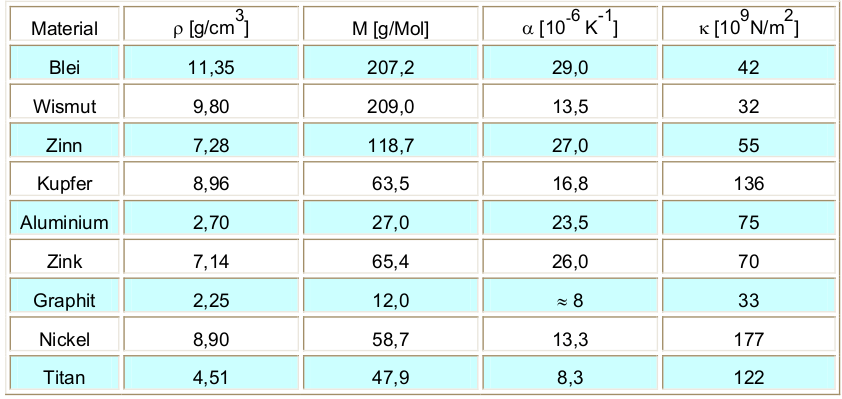
\includegraphics[height=5cm]{logos/tab.png}
  \caption{Physikalische Eigenschaften der Probemateriallien \cite{Anleitung}}
  \label{fig:tab}
\end{figure}
Die Materialkonstanten der Probekörper sind in der Tabelle in
Abbildung \ref{fig:tab} dargestellt.
Im Folgenden wird die Temperatur mit einem Thermoelement gemessen, welches
an ein Digitalvoltmeter angeschlossen ist. Die so gemessene Spannung $U$
steht mit der Temperatur $T$ in folgendem Zusammenhang:
\begin{equation}
  T = a\cdot U + b \,.
  \label{eqn:TU}
\end{equation}
Hier bezeichnen $ a $ und $b$ einfache Konstanten.


























%
